\documentclass[12pt, a4paper]{report}

\usepackage[margin=20mm]{geometry}
\usepackage{calc}
\usepackage[default]{sourcesanspro}
\usepackage{tikz}
\usepackage{etoolbox}
\usepackage{hyperref}
\usepackage[none]{hyphenat}
\usepackage{amssymb}
\usepackage{amsmath}
\usepackage{longtable}
\usepackage{booktabs}
\usepackage{fancyhdr}
\usepackage[toc]{glossaries}
\usepackage[lofdepth,lotdepth]{subfig}
\usepackage{graphicx}

\usepackage{float}
\floatplacement{figure}{h}

\usepackage{xcolor}
\definecolor{white}{HTML}{FFFFFF}
\definecolor{black}{HTML}{000000}
\definecolor{green}{HTML}{198701}
\definecolor{orange}{HTML}{FF6138}
\definecolor{red}{HTML}{ba0900}
\definecolor{blue}{HTML}{0B75CB}
\definecolor{yellow}{HTML}{EFC82B}
\definecolor{purple}{HTML}{49075E}
\definecolor{webpage}{HTML}{a18613}
\colorlet{primary}{webpage}
\newcommand{\primary}[0]{\color{primary}}
\newcommand{\black}[0]{\color{black}}

\usetikzlibrary{shapes.geometric, arrows, fit}
\tikzstyle{process} = [rectangle, minimum width=3cm, minimum height=1cm, text centered, draw=black, fill=orange!30]
\tikzstyle{page} = [rectangle, minimum width=3cm, minimum height=1cm, text centered, draw=black, fill=primary!30, rounded corners=4pt]
\tikzstyle{menu} = [rectangle, minimum width=3cm, minimum height=1cm, text centered, draw=black, fill=purple!30, rounded corners=4pt]
\tikzstyle{group} = [rectangle, minimum width=3cm, minimum height=1cm, text centered, draw=black, thick]
\tikzstyle{arrow} = [thick,<->,>=stealth]

\usepackage[colorinlistoftodos,color=primary]{todonotes}

\usepackage{framed}
\usepackage[framemethod=TikZ]{mdframed}
\newcounter{note}\setcounter{note}{0}
\renewcommand{\thenote}{\arabic{note}}
\newenvironment{note}[1]{
	\begin{minipage}{\linewidth}
		\vspace{1em}
		\stepcounter{note}
		\ifstrempty{#1}{
			\mdfsetup{
				frametitle={
					\tikz[baseline=(current bounding box.east),outer sep=0pt]
					\node[anchor=east,rectangle,fill=primary!20]
					{\strut Note~\thenote};
				}
			}
		}{
			\mdfsetup{
				frametitle={
					\tikz[baseline=(current bounding box.east),outer sep=0pt]
					\node[anchor=east,rectangle,fill=primary!80,rounded corners=4pt]
					{\strut~#1};
				}
			}
		}
		\mdfsetup{roundcorner=10pt,innertopmargin=0pt,linecolor=primary!80,linewidth=2pt,topline=true,frametitleaboveskip=\dimexpr-\ht\strutbox\relax}
		\begin{mdframed}[]\relax
		}{
	\end{mdframed}\end{minipage}
}
\renewenvironment{leftbar}[1][\hsize]
{
    \def\FrameCommand
    {
        {\color{primary}\vrule width 2pt}
        \hspace{0pt}%must no space
        \fboxsep=\FrameSep\colorbox{primary!10}
    }
    \MakeFramed{\hsize#1\advance\hsize-\width\FrameRestore}
}
{\endMakeFramed}

\newcommand{\persona}[5]{
	\begin{note}{#1}
		\begin{description}
			\item[Age:] #2
			\item[Gender:] #3
			\item[Goals:]
			\item[]#4
			\item[Pain Points:]
			\item[]#5
		\end{description}	
	\end{note}
}

% set the title format
\usepackage[explicit]{titlesec}
% \usepackage{xhfill}
\newcommand{\vrulefill}[1]{\leavevmode\leaders\hrule height#1\hfill\kern0pt}
\newcommand{\firstletter}[1]{\primary#1\black}
\newcommand{\ruleafter}[1]{#1~\xrfill[.7ex]{1pt}}
\titleformat{\section}{\bfseries\primary\Large}{\thesection}{0.75em}{#1\quad\vrulefill{0.12em}}
\titlespacing*{\section}{0em}{3em}{0em}
\titleformat{\subsection}{\bfseries\primary\large}{\thesubsection}{0.75em}{#1}
\titlespacing*{\subsection}{0em}{1em}{0em}
\def\myfirstletter#1{\primary#1\black}
\DeclareRobustCommand{\FirstPrimaryLetter}[1]{\myfirstletter #1}
\titleformat{\subsubsection}[hang]{\bfseries\large}{}{0em}{\quad\FirstPrimaryLetter#1}
\titlespacing*{\subsubsection}{0em}{1em}{0em}
\setcounter{secnumdepth}{3}
\renewcommand\contentsname{Table of Contents}
\setlength\parindent{0pt}

% set the item spacing
\usepackage{enumitem}
\setlist{nosep}

\fancyfoot{}
\fancyhead{}
\fancyhead[L]{\leftmark}
\fancyhead[R]{\rightmark}
%\fancyhead[C]{Design Report}
\fancyfoot[R]{Page\ \thepage}
\fancyfoot[L]{DECO1400}
\fancyfoot[C]{Daniel Fitzmaurice (\primary 43961229\black)}
\renewcommand{\headrulewidth}{0.15em}
\renewcommand{\footrulewidth}{0.15em}
\renewcommand{\headrule}{\hbox to\headwidth{\primary\leaders\hrule height\headrulewidth\hfill}}
\renewcommand{\footrule}{\hbox to\headwidth{\primary\leaders\hrule height\footrulewidth\hfill}}

\makeglossaries
\newacronym{api}{API}{Application Programming Interface}
\newglossaryentry{javascript}{
	name={JavaScript},
	description={Browser scripting language used to provide interactive features}
}
\newglossaryentry{react}{
	name={React},
	description={JavaScript framework which utilizes the virtual DOM and component based tree structure to improve application performance and reduce code duplication}
}
\newglossaryentry{typescript}{
	name={TypeScript},
	description={Adds static type checking to JavaScript}
}
\newglossaryentry{smarthome}{
	name={SmartHome},
	description={An environment in which a series of different devices communicate and interact together to provide an end user with a more automated housing experience}
}
\newglossaryentry{git}{
	name={Git},
	description={A popular version control system for tracking a change history of code and providing easily collaboration between developers. Git is commonly used with an online public repository such as GitHub or GitLab}
}

\begin{document}
	% !TeX spellcheck = en_US
% !TeX root = main.tex
\begin{titlepage}
\begin{center}

\begin{minipage}{\textwidth}
	\begin{center}
		\begin{minipage}{\widthof{\Huge Daniel Fitzmaurice}}
			\Huge
			Daniel Fitzmaurice\\
			\vspace{1em}
			\hfill(43961229)\\
		\end{minipage}
	\end{center}
	\vspace{10em}
\end{minipage}
\begin{minipage}{\textwidth}\begin{center}
		\includegraphics{logo}\\\vspace{0em}
		\huge University of Queensland\\
		\LARGE\color{primary}\textbf{DECO1400}\color{black}\ -- Design Computing\\\vspace{2em}
		Final Report Thingy
\end{center}\end{minipage}

\begin{tikzpicture}[remember picture,overlay,shorten >= -10pt]
	\coordinate (aux1) at ([yshift=-15pt]current page.north east);
	\coordinate (aux2) at ([yshift=-410pt]current page.north east);
	\coordinate (aux3) at ([yshift=-4.5cm]current page.north east);
	\coordinate (aux4) at ([yshift=-150pt]current page.north east);
	
	\begin{scope}[primary!40,line width=12pt,rounded corners=12pt]
		\draw
			(aux1) -- coordinate (a)
			++(225:5) --
			++(-45:5.1) coordinate (b);
		\draw[shorten <= -10pt]
			(aux3) --
			(a) --
			(aux1);
		\draw[opacity=0.6,primary,shorten <= -10pt]
			(b) --
			++(225:2.2) --
			++(-45:2.2);
	\end{scope}
	\draw[purple,line width=8pt,rounded corners=8pt,shorten <= -10pt]
		(aux4) --
		++(225:0.8) --
		++(-45:0.8);
	\begin{scope}[primary!70,line width=6pt,rounded corners=8pt]
		\draw[shorten <= -10pt]
			(aux2) --
			++(225:3) coordinate[pos=0.45] (c) --
			++(-45:3.1);
		\draw
			(aux2) --
			(c) --
			++(135:2.5) --
			++(45:2.5) --
			++(-45:2.5) coordinate[pos=0.3] (d);
		\draw
			(d) -- +(45:1);
	\end{scope}
\end{tikzpicture}

\end{center}
\end{titlepage}
	\newpage
	\pagenumbering{roman}
	\tableofcontents
	\listoffigures
	%\listoftables
	\printglossary
	\newpage
	
	\pagestyle{fancy}
	\pagenumbering{arabic}
	
	\chapter{Design and Details}
	% !TeX spellcheck = en_US
% !TeX root = main.tex

\section{Introduction}
% Who and what is this design report for?
% What can we expect from the follow pages?
\todo[inline]{Need to revisit this}

This design report is used to describe the process used to design and develop a website for teaching and instructing people of how version control systems work and the typical process flow of \gls{git}.

\subsection{Introduce Yourself}
% Briefly describe yourself
% What's your background?
% What's your skills, interests, degree, etc
% What's your learning strategy (as defined in the Week 1 practical) at the start of the course
I am currently studying in my fifth year of Engineering majoring in Software at the University of Queensland. My expertise is in low level computing as well as website application development, using modern frameworks such as \gls{react} and \gls{typescript}. I have completed my thesis under the supervision of Alex Pudmenzky where I designed and constructed a website and mobile application which interfaced with a series of different \gls{smarthome} applications. I am currently working as a developer at Aurecon where my knowledge of \gls{react} and \gls{javascript} are used to develop applications and work extensively with industry \gls{api}s.

\subsubsection{Learning Strategy}
Even though I have quite strong experience in JavaScript and website development, a lot of my experience has been through using frameworks and early release technologies. So my strategy is to create a well document which has good accessibility design and is supported incredibly well across all system. All features as well as most bonus features should be usable on all platforms.\\\\
Across my development I have not had much experience with the design phase of a project either, so it a goal of mine to embrace the design and learn as much as I can about the processing and thought procedures involved with designing and a website and not just jumping in immediately and developing.
	% !TeX spellcheck = en_US
% !TeX root = main.tex

\section{Getting to Know Stakeholders}
\subsection{Target Audience}
% Who is the specific target audience in relation to the brief?
% Include a few personas that represent different, archetypal users
% What are some common traits you've identified from your personas?
% What implications does this audience have for the design?
It is always essential to pick a target audience for a project before beginning, this will help to identify relevant content and ideas that should or should not be used. For this project the target audience is centred around people just beginning to learn about code or beginning to enter a professional environment where their code or actions will be marked and versioned. These sorts of people at typically around 18 to 22 years old and have some basic experience with computers and know how to work their way around the system. However they are still incredibly knew to the environment and if content is not broken down in an understandable way then they can be easily confused and lose interest.

\subsubsection{Goals}
With the target audience specified it can now be import to outline goals that should be followed to ensure the target audience is engaged.
\todo[inline]{Get all the references}
\begin{description}
	\item[Consumable Chunks:] The target audience require information to be broken down into consumable chunks in which they can learn, reflect, and then use before moving on to the next chunk.
	\item[Direct Content Flow:] Content chunks should also logically flow from one section to the next without large gaps in presentation. Not following this goal will ultimately result in the consumer losing track and becoming disinterested.
	\item[Simplistic Graphics:] Following design patterns released by large web driven companies, such as Google and Facebook, content should be shown in a way that is not overcrowded and can be confusing. If graphics are used to illustrate a point they should be vector based to help provide a more defining and clean look.
	\item[Defined Website Theme:] In order to engage the users and not make them lose interest, the website must have a clear and engaging theme that is applied site wide. This will help to reduce confusion about different sections of the site.
	\item[Clean and Polished:] The site as a whole should be clean and usable site. This means performance should remain consistent and have an expected behaviour across the entire site. As well all graphics should be presented in a high quality and consistent manor, this can be achieved using vector graphics and rendering on the client side. Finally the site should function across all modern browsers and devices, as well as having accessibility support.
\end{description}


\subsection{Chosen Educational Content}
% What is your chosen educational content?
% Why is this educational content an interesting choice for the target audience?
For this website, the goal is to be a resource for people wanting to learn about git the version source control system. Git allows people to track and mark changes they are making to code as well as easily allowing other people to integrate and edit the code together. Git fits well into the target audience because it is becoming more and more essential programming jobs and is becoming assumed knowledge for every programmer. Therefore people just starting in industry might not have knowledge about this tool and therefore need to upskill quickly and efficiently.

\subsection{Chosen Story}
% What is your chosen story and genre?
% Why is this story an interesting choice for the website's visuals and theme in relation to the target audience?
\todo[inline]{Find a story}
	% !TeX spellcheck = en_US
% !TeX root = main.tex

\section{Navigation and Organisation}
\subsection{Card Sorting}
% Reflect on the success of the Card Sorting design activity you did in Week 4
% Include the testing plan you developed for the activity
% Include photos you took of the activity running
% What feedback did you get and how did it inform your early content organisation decisions?
% Which organisation systems will you use in your website and why?

\subsubsection{The Plan}
To begin there were three main areas of content were identified: Git Reference Summary, Main storyline/tutorial, Interactive Quiz. These areas were then assigned a rank and associated keywords:
\begin{itemize}
	\item\textbf{Git Reference Summary}
	\begin{itemize}
		\item Shows all the commands and a basic overview of what they do
		\item This will be visited most by people coming back because they forgot something or wanted to know more outside of the main storyline
		\item \textbf{Rank:} 2
		\item \textbf{Keywords:} Advanced, Reflection, Quick
	\end{itemize}
	\item\textbf{Main storyline/tutorial}
	\begin{itemize}
		\item This will be most frequently visited by new comers and people just visiting the site
		\item \textbf{Rank:} 1
		\item \textbf{Keywords:} Beginner, Interesting, Interactive
	\end{itemize}
	\item\textbf{Interactive Quiz}
	\begin{itemize}
		\item Some of this will also be embedded inside the storyline
		\item People wanting a challenge and to learn more
		\item \textbf{Rank:} 3
		\item \textbf{Keywords:} Self Learning, Interactive, All Levels
	\end{itemize}	
\end{itemize}

For this survey I chose to go with an Open Card Sort because I wanted to observe how they thought about grouping and what is easier or more important to sort before arriving at a final decision. After the users had finished with sorting the cards, a couple of follow up questions/discussions would be had around why they named the groups they did.

\subsubsection{Execution}
In order to execute the card sorting, Trello was used for the physical moving of cards around. This decision was made because it best allows people to move the cards around like they would physically, while still providing them with the easy of changing the names of the groups.

\subsubsection{Results}
\begin{note}{Person 1}
	\begin{figure}[H]
		\centering
		\includegraphics[width=\linewidth]{card1}	
		\caption{Person 1's Card Sorting Result}
	\end{figure}

	How did you group the tags?
	\begin{leftbar}
		Beginner and advanced are varying difficulties, I don't know if that is something I can choose. All levels are associated, can I filter by difficulty level on the side.\\\\
		Grouped them because the concepts are the same, but on the site I wouldn't expect beginner and advance to be together.
	\end{leftbar}

	How did you name the groups?
	\begin{leftbar}
		\begin{itemize}
			\item Difficulty
			\begin{itemize}
				\item When you play a video game you pick your difficulty level
			\end{itemize}
			\item Learnability
			\begin{itemize}
				\item Self learning, learnability makes sense
				\item Interactive is key to learning
				\item Reflection is key to learning, gauge how successful you were
			\end{itemize}
			\item Fun Factor
			\begin{itemize}
				\item Interactive website's are fun, reading a static page can be quite passive and boring
				\item It's interesting because I am curious and it feels more tactile
			\end{itemize}
			\item How in Depth (\textit{mean not very in depth})	
			\begin{itemize}
				\item I would go through the site really quickly
				\item So the level of detail in the website is probably really shallow
			\end{itemize}
		\end{itemize}
	\end{leftbar}
\end{note}

\begin{note}{Person 2}
	\begin{figure}[H]
		\centering
		\includegraphics[width=\linewidth]{card2}	
		\caption{Person 2's Card Sorting Result}
	\end{figure}

	How did you group the tags?
	\begin{leftbar}
		Beginner and advanced are linked and interesting is cool\\\\
		All Levels and Quick are navigation type\\\\
		Reflection/SL/Interactive seem like quizzing	
	\end{leftbar}
	
	How did you name the groups?
	\begin{leftbar}
		\begin{itemize}
			\item Quiz/Review
			\begin{itemize}
				\item Reflection/SL is like looking back at what you learnt
				\item Looking back
			\end{itemize}
			\item Info
			\begin{itemize}
				\item Looking at Beginner and Advanced and interactive is like the middle of where you go
				\item Middle man of the navigation
			\end{itemize}
			\item Home
			\begin{itemize}
				\item They seem like navigation and be able to go through the site
			\end{itemize}
		\end{itemize}
	\end{leftbar}
\end{note}



\subsection{Navigation Systems}
% What were the key things you learned from your Navigation Systems group discussion?
% Write a brief response of your own to the guiding questions for this group discussion
% Which navigation systems will you use in your website and why?
A lot of the shown ``correct'' styles of navigation systems followed a similar style and placement. A lot of ``incorrect'' styles were outside the norm of having common elements. These elements are:
\begin{itemize}
	\item A main banner which include a general logo and quick navigation links underneath
	\item Most of the examples also used an inner page navigation panel on the left for filtering content on the current page	
\end{itemize}\vspace{1em}
Reflecting on the themes and the presentation styles used across websites that are considered good design, a similar layout will be used for this website. However slight modifications will be made to suit a scrolling storyline layout. To increase screen size and make the website appear more story like, the main logo will be reduced to be inline with the primary navigation menu. A side navigation menu will be created but it will be semi-hidden for a majority of the website and only showing itself when the mouse interacts with the shown tip.


\subsection{Site Map}
% Draw a site map that visualises the navigation flow of your website
% Include any internal (between pages) and external links
% Storyboard how one of your personas will navigate your website
\begin{figure}
	\centering
	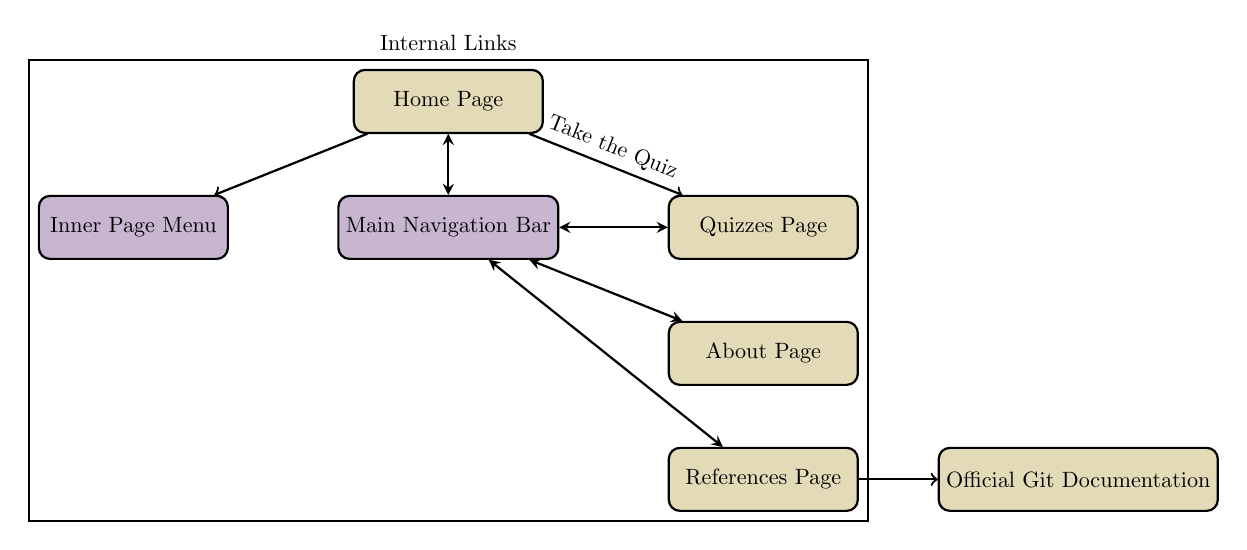
\begin{tikzpicture}[node distance=2cm,thick,every node/.style={scale=0.8}]
		\node (main) [page] {Home Page};
		\node (menu) [menu, below of=main] {Main Navigation Bar};
		\node (quiz) [page, right of=menu,xshift=3cm] {Quizzes Page};
		\node (about) [page, below of=quiz] {About Page};
		\node (refs) [page, below of=about] {References Page};
		
		\node (innerMenu) [menu, left of=menu,xshift=-3cm] {Inner Page Menu};
		
		\node (externalGit) [page, right of=refs,xshift=3cm] {Official Git Documentation};
		
		\node (internal) [group, fit=(main) (menu) (refs) (quiz) (about) (innerMenu),label={Internal Links},scale=1.25] {};
		
		\draw [arrow] (main) -- (menu);
		\draw [arrow] (menu) -- (refs);
		\draw [arrow] (menu) -- (quiz);
		\draw [arrow] (menu) -- (about);
		\draw [->] (main) -- (innerMenu);
		\draw [->] (refs) -- (externalGit);
		\draw [->] (main) -- node [midway,above,rotate=-22]{Take the Quiz} (quiz);
	\end{tikzpicture}
	\caption{Site Map Navigation}\label{fig:sitemap}
\end{figure}

\subsubsection{Site Map Navigation}
The site map design is shown in Figure~\ref{fig:sitemap}, here the user will enter the site via the ``Home Page'' which will be the main story page. Then to navigate they can chose to navigate through the home page using the ``Inner Page Menu'' or via scrolling. The other main navigation feature will the be top bar which can be used to navigate to the other pages within the site (``Quizzes Page'', ``About Page'', ``References Page''). From these pages, the same navigation element will exist allowing the user to navigate back or to other pages as they see required.\\\\

There will be small link at the bottom of the home page what will direct the user to the quizzes page, this symbolises that they have all the knowledge they require and it is time to see if they really learnt as much or need to go back through and understand it much more clearly.


\subsection{Visual Organisation}
% What were the key things you learned from you Visual Organisation group discussion?
% Write a brief response of your own to the guiding questions for this group discussion

\begin{figure}
	\centering
	\includegraphics[width=\linewidth]{ubuntu}
	\caption{Screenshot of Ubuntu Desktop webpage}\label{fig:ubuntu}
\end{figure}

The example site picked for the visual organisational layout is the Ubuntu Desktop webpage (Figure~\ref{fig:ubuntu}). This site incorporates a lot of good design choices and creates a very pleasant user experience through its choice in positioning and colors.

\subsubsection{Spacing}
The page utilises a lot of spacing around elements to signify the beginning and ending of different sections and content. And pictures are used to help create this space without making the space seem stretched out or the significance of ``white space''.

\subsubsection{Colours and Fonts}
Ubuntu has used a very basic colour palette here, simply just black and white with orange as a primary colour. The use and choice of colour has resulted in the images having a really attention drawn in factor and the text combined with the font choice, is easy and delightful to read. A user is draw to the picture foremost and then curiosity about what they are looking at draws them into the text to find out more. The styling of the text creates a calm and informal attitude which invites readers to only view the information they think is relevant.

\subsubsection{Alignment and Layout}
The webpage appears to use a three column approach where either content is split across three columns, or the image consumes two columns and text is floated left or right of the image. However due to the use of spacing, this column structure is not strict and instead boosts the appearance of a relax and informal presentation.

\subsubsection{Weight}
Ubuntu has taken a none-traditional approach to weight in web design by not so much assigning weighting to how bold or coloured the text is. Instead an approach of providing spacing and increased font size is favoured, however font weighting is still used. This primarily puts focus around the user seeing the larger text and the proceeding white space around it as a reference for the weight of a piece of text. This unique approach has provided Ubuntu with the relaxed and informal vibe that appears to be the design goal behind the entire site.


\subsection{Interactivity and Functionality}
% Draw wireframes for each type of page in your website (i.e. if you have 5 pages that function very similarly, you only need to draw 1 wireframe)
% These can be derived from the same mockups you produced for Paper Prototyping
% Add annotations to describe:
% - how each interactive element functions
% - how they are designed to engage your specific target audience
% - how they are designed to strengthen the educational content
% - and how you think it will be implemented at this stage (HTML, CSS or JavaScript)

\subsection{Paper Prototyping}
% Reflect on the success of the Paper Prototyping design activity you did in Week 6
% Include photos/screenshots of your paper prototypes
% Include the testing plan you developed for the activity
% Include photos you took of the activity running
% What feedback did you get and how did it inform your visual organisation, navigation and functionality decisions?
\begin{figure}
	\centering
	\includegraphics[width=0.8\linewidth]{rainy}
	\caption{User completing the paper prototype test}
\end{figure}

The paper prototype was broken up into the following tests:

\subsubsection{Learn the Basics}
\begin{itemize}
	\item\textbf{Do:} ``Learn the basics''
	\item\textbf{Watch:} If they scroll through the homepage or jump to references
	\begin{itemize}
		\item\textbf{Person 1:} Hovered over the code snippet. Hovered over the heading. ``Will I be looking at whitespace''
		\item\textbf{Person 2:} Went to the about page first
	\end{itemize}
	\item\textbf{Ask:}
	\begin{itemize}
		\item ``Was it intuitive to scroll	the page?''
		\begin{itemize}
			\item\textbf{Person 1:} Yeah very intuitive, but there is no menu have to scan the entire page
			\item\textbf{Person 2:} Yes it was quite intuitive, I think that normally when someone encounters a website they would scroll down for more information. Especially when the title says getting started
		\end{itemize}
		\item ``Do you feel like the content is will spaced out?''
		\begin{itemize}
			\item\textbf{Person 1:} Yeah but vertical spacing is verging on a little too much
			\item\textbf{Person 2:} If each section is separated then yes, otherwise separate pages might be effective
		\end{itemize}
	\end{itemize}
\end{itemize}


\subsubsection{Complete the Quiz}
\begin{itemize}
	\item\textbf{Do:} ``Complete the Quiz''
	\item\textbf{Watch:} How capable each of the controls in the quiz are
	\begin{itemize}
		\item\textbf{Person 1:} Got really confused about the terminal thing
	\end{itemize}
	\item\textbf{Ask:}
	\begin{itemize}
		\item ``Did you feel like it was obvious there was a quiz?''
		\begin{itemize}
			\item\textbf{Person 1:} Yeah it was obvious because of the quiz button. Weird it was between references and about
			\item\textbf{Person 2:} Yes because there was a heading up the top saying quiz
		\end{itemize}
		\item ``Was the Quiz easy to flow through?''
		\begin{itemize}
			\item\textbf{Person 1:} I don't know how many questions there are... Yes
			\item\textbf{Person 2:} Yes
		\end{itemize}
		\item ``Do you think you would benefit from the quiz?''
		\begin{itemize}
			\item\textbf{Person 1:} Yes cause I know what I don't know, find out weak spots
			\item\textbf{Person 2:} Yes because a quiz is useful to check whether the content learnt was absorbed
		\end{itemize}
	\end{itemize}	
\end{itemize}


\subsubsection{Get information on Advanced commands}
\begin{itemize}
	\item\textbf{Do:} ``Get information on Advanced commands''
	\item\textbf{Watch:} If they scroll through the home page screen first or go straight to the references page
	\begin{itemize}
		\item\textbf{Person 1:} Went to the homepage first
		\item\textbf{Person 2:} Went to the homepage first
	\end{itemize}
	\item\textbf{Ask:}
	\begin{itemize}
		\item ``Was it clear that there is a references overview page?''
		\begin{itemize}
			\item\textbf{Person 1:} Yeah but I thought it was citations, not git command references
			\item\textbf{Person 2:} Yes there was a title at the top saying references. Title it ``git command reference''
		\end{itemize}
	\end{itemize}	
\end{itemize}


\subsubsection{View information about the creator}
\begin{itemize}
	\item\textbf{Do:} ``View information about the site creator''
	\item\textbf{Watch:} How easy the navigation bar is to use
	\item\textbf{Ask:}
	\begin{itemize}
		\item ``Did you know exactly where you wanted to go?''
		\begin{itemize}
			\item\textbf{Person 1:} yeah but thought about was about the page not about the person
			\item\textbf{Person 2:} yes this was a very intuitive button
		\end{itemize}
	\end{itemize}	
\end{itemize}


\subsubsection{How do you update your git?}
\begin{itemize}
	\item\textbf{Do:} ``How do you update your git repo?''
	\item\textbf{Watch:} If they navigate to the references or the home page
	\begin{itemize}
		\item\textbf{Person 1:} Navigated to the home page
		\item\textbf{Person 2:} Navigated to the references page	
	\end{itemize}
	\item\textbf{Ask:}
	\begin{itemize}
		\item ``Did you know where you needed to go?''
		\begin{itemize}
			\item\textbf{Person 1:} Yeah I had a vague idea because I started on that page. I wouldn't if I didn't scroll the page
			\item\textbf{Person 2:} Yes, because the references will show me all the commands I can use
		\end{itemize}
	\end{itemize}	
\end{itemize}

\begin{figure}
	\centering
	\subfloat[Paper Prototype screen of the main homepage]{
		\includegraphics[width=0.5\textwidth,angle=-90,origin=c]{paper2}\label{fig:paper2}}
	\qquad
	\subfloat[Paper Prototype screen of the references page]{
		\includegraphics[width=0.5\textwidth,angle=-90,origin=c]{paper1}\label{fig:paper1}}

	\caption{Screenshots of paper prototype}
	\label{fig:paper}
\end{figure}


	
	\chapter{Development and Implementation}
	% !TeX spellcheck = en_US
% !TeX root = main.tex

\section{Aesthetics}
\subsection{Style Guide}
% Summarise the general aesthetic you've chosen and your design intentions
% How does your visual aesthetic engage your specific target audience?
% Visualise (with contextual examples):
% - Which color scheme did you use? Include HEX codes
% - Describe your text treatments. Include font names, sizes and weights
% - Describe any image or icon treatments
% - Describe any button/link treatments (e.g. hovering on a link)
% Rationalise the design choices you've made, relating to the design principles from the lectures

% https://www.verywellmind.com/color-psychology-2795824

\subsection{Aesthetics User Testing}
% Reflect on the success of the Aesthetics User Testing design activity you did in Week 9
% Include screenshots of the mockups you used for the activity
% Include the testing plan you developed for the activity
% What feedback did you get and how did it inform your aesthetic decisions?
	% !TeX spellcheck = en_US
% !TeX root = main.tex

\section{Website Implementation}
\subsection{Accessibility, Graceful Degradation \& Progressive Enhancement}
% What were the key things you learned from your Accessibility, Graceful Degradation and Progressive Enhancement group discussions?
% Write brief responses of your own to the guiding questions for these group discussions
% Rationalise why you've chosen to use JavaScript instead of HTML hyperlinks or CSS features of your website
% How has your website used a combination of HTML, CSS and JavaScript to great effect?

\subsection{Security \& Privacy}
% What were the key things you learned from your Security \& Privacy group discussions?
% Write brief responses of your own to the guiding questions for these group discussions

\subsection{Hi-Fi User Testing}
% Reflect on the success of the Hi-Fi User Testing design activity you did in Week 13
% Include the testing plan you developed for the activity
% Include photos you took of the activity running
% What feedback did you get and how did it inform your final product?
	
	% !TeX spellcheck = en_US
% !TeX root = main.tex

\chapter{Conclusion}
% Summarise and conclude your Design Report
% In short, how has your website been successful in responding to the brief?

\section{Course Reflection}
% How has your learning strategy changed since the start of the course?
% If you had the change to restart, how would you approach your learning differently?
	
	\newpage
	\addcontentsline{toc}{chapter}{References}
	\bibliographystyle{ieeetr}
	\bibliography{bib}
	
\end{document}